\documentclass[10pt,twocolumn]{article}

\usepackage[margin=0.76in,columnsep=0.22in]{geometry}
\usepackage[T1]{fontenc}
\usepackage[utf8]{inputenc}
\usepackage{lmodern}
\usepackage{microtype}
\usepackage{graphicx}
\usepackage{booktabs}
\usepackage{tabularx}
\usepackage{array}
\usepackage{amsmath,amssymb}
\usepackage{enumitem}
\usepackage{caption}
\usepackage{subcaption}
\usepackage{xcolor}
\usepackage{url}
\usepackage[hidelinks]{hyperref}

\hypersetup{
  pdftitle={Multimodal Sensor Fusion for Human Activity Recognition on Adapted MHEALTH},
  pdfauthor={Satya Siddhartha Balanagu},
  pdfsubject={Assignment 2 Technical Report},
  pdfkeywords={MHEALTH, multimodal fusion, activity recognition, inertial sensors, deep learning, GDPR, AI ethics}
}

\graphicspath{{figures/}}
\captionsetup{font=small,labelfont=bf,skip=3pt}
\setlist{nosep,leftmargin=*}
\setlength{\parindent}{1em}
\setlength{\parskip}{0pt}
\renewcommand{\arraystretch}{1.08}
\makeatletter
\setlength{\@fptop}{0pt}
\setlength{\@dblfptop}{0pt}
\makeatother

\newcolumntype{Y}{>{\raggedright\arraybackslash}X}
\newcolumntype{Z}{>{\centering\arraybackslash}X}

\title{\textbf{Multimodal Sensor Fusion for Human Activity Recognition:}\\
\large Exploring Data-Level and Decision-Level Fusion across Inertial Modalities on Adapted MHEALTH}

\author{
Satya Siddhartha Balanagu\\
Student ID: A1961325\\
School of Computer Science, University of Adelaide
}

\date{28 September 2026}

\begin{document}


\renewcommand{\topfraction}{0.95}
\renewcommand{\bottomfraction}{0.95}
\renewcommand{\textfraction}{0.05}
\renewcommand{\floatpagefraction}{0.75}
\renewcommand{\dbltopfraction}{0.95}
\renewcommand{\dblfloatpagefraction}{0.75}


\setlength{\textfloatsep}{6pt plus 1pt minus 2pt}
\setlength{\dbltextfloatsep}{6pt plus 1pt minus 2pt}
\setlength{\floatsep}{5pt plus 1pt minus 1pt}
\setlength{\dblfloatsep}{5pt plus 1pt minus 1pt}
\setlength{\intextsep}{5pt plus 1pt minus 1pt}

\maketitle

\begin{abstract}
Human Activity Recognition (HAR) using wearable inertial and physiological sensing is fundamental to pervasive digital health, elderly tele-monitoring, and sports biomechanics. However, single-sensor modalities invariably suffer from anatomical blind spots, spatial occlusion, and noise susceptibility. This technical report presents an end-to-end multimodal machine learning pipeline on the adapted Mobile HEALTH (MHEALTH) benchmark dataset. We first conduct an in-depth exploratory data analysis (EDA) across 343,195 observations from 10 volunteers, uncovering physical energy stratifications across 12 discrete activities and low cross-modal kinematic redundancy. We comprehensively audit 615,648 missing values (7.80\% overall missingness) caused by wireless packet dropouts, proving that 92.4\% of bursts span only a single sample (20\,ms) and establishing a segment-bounded intra-run linear interpolation strategy that strictly eliminates cross-activity and cross-participant boundary contamination. We select three anatomically distributed sensor sources spanning two distinct physical modalities: Chest Accelerometer (trunk posture), Left-Ankle Accelerometer (lower-limb impact dynamics), and Right-Wrist Gyroscope (upper-limb angular rotational rates). To ensure unbiased real-world generalisation, we enforce a strict subject-independent partitioning scheme (Training: Subjects 1--7; Validation: Subject 8; Testing: Subjects 9--10). Under identical training budgets, optimisers, and cosine annealing schedules, we evaluate three unimodal baselines against two multimodal fusion paradigms: Data/Feature-Level Early Fusion and Decision-Level Late Soft-Voting. Experimental results demonstrate that multimodal fusion decisively outperforms all unimodal baselines, boosting test accuracy from 85.60\%--88.50\% to 95.56\% and Macro-F1 from 0.8253--0.8848 to 0.9568 (+7.2\% to +13.1\% absolute improvement). Crucially, fusion completely resolves unimodal failure modes, eliminating confusion between walking, stair climbing, arm elevations, and explosive jumping. Finally, we provide an exhaustive analysis of computational edge trade-offs, showing that on-node feature extraction achieves an 85.3\% telemetry bandwidth reduction, and propose a comprehensive regulatory governance matrix adhering to GDPR Articles 4, 9, and 22, HIPAA, and Australian Privacy Principles.
\end{abstract}

%%%%%%%%%%%%%%%%%%%%%%%%%%%%%%%%%%%%%%%%%%%%%%%%%%%%%%%%%%%%%%%%%%%%%%%%%%%%%%%%
% SECTION 1: TASK 1 - DATA EXPLORATION
%%%%%%%%%%%%%%%%%%%%%%%%%%%%%%%%%%%%%%%%%%%%%%%%%%%%%%%%%%%%%%%%%%%%%%%%%%%%%%%%
\section{Task 1: Data Exploration}
\label{sec:task1}

\subsection{Dataset Provenance and Architecture}
The Mobile HEALTH (MHEALTH) dataset, originally collected by Ba{\~n}os et al.~\cite{banos2014mhealthdroid,banos2015sensor} and archived in the UCI Machine Learning Repository~\cite{mhealth_uci_2014}, serves as an established benchmark for multimodal pervasive sensing. The dataset captures continuous body motion and vital signs across ten healthy adult volunteers (6 male, 4 female; aged 20--35) executing an extensive repertoire of daily living activities and calisthenic exercises in an unconstrained out-of-laboratory setting. 

Sensing is performed using three synchronised Shimmer2 wearable inertial units attached securely via elastic straps to three distinct anatomical sites:
\begin{enumerate}
    \item \textbf{Chest (Trunk):} Captures gross upper-body orientation, postural inclination, respiratory/cardiac vibrations, and spinal flexion via a tri-axial accelerometer ($\pm 1.5\,\text{g}$ range, $\text{m/s}^2$) and a 2-lead electrocardiogram (ECG, $\text{mV}$).
    \item \textbf{Left Ankle (Lower Extremity):} Measures ground reaction impacts, propulsion forces, and ambulatory stepping frequency via a tri-axial accelerometer ($\pm 6\,\text{g}$ range), a tri-axial gyroscope ($\pm 500^\circ/\text{s}$ range), and a tri-axial magnetic sensor ($\pm 1\,\text{local field}$).
    \item \textbf{Right Wrist (Upper Extremity):} Monitors fine-grained upper-limb manipulations, dynamic arm swings, and rotational gestures via a tri-axial accelerometer, a tri-axial gyroscope, and a tri-axial magnetometer.
\end{enumerate}
All sensing modalities are uniformly recorded at a continuous sampling frequency of $f_s = 50\,\text{Hz}$ ($\Delta t = 20\,\text{ms}$), providing adequate Nyquist coverage for human biomechanical motion ($<20\,\text{Hz}$)~\cite{bulling2014tutorial}.

\begin{table*}[t]
\centering
\small
\caption{Taxonomy of activities, duration/repetitions, kinetic categorization, and segmented 2.56-second window counts in the adapted MHEALTH dataset ($N=5,229$ windows across 10 participants).}
\label{tab:activities}
\begin{tabularx}{\textwidth}{clllcc}
\toprule
\textbf{ID} & \textbf{Activity Name} & \textbf{Nominal Protocol} & \textbf{Kinetic Classification} & \textbf{Raw Samples} & \textbf{Windows ($W=128$)} \\
\midrule
$L_1$ & Standing still & 1 min timed & Static Postural Balance & 30,720 & 470 \\
$L_2$ & Sitting and relaxing & 1 min timed & Static Sedentary Posture & 30,720 & 470 \\
$L_3$ & Lying down & 1 min timed & Static Recumbent Posture & 30,720 & 470 \\
$L_4$ & Walking & 1 min timed & Rhythmic Ambulatory Locomotion & 30,720 & 470 \\
$L_5$ & Climbing stairs & 1 min timed & Inclined Ambulatory Stepping & 30,720 & 470 \\
$L_6$ & Waist bends forward & 20 repetitions & Trunk Flexion / Calisthenic & 28,315 & 429 \\
$L_7$ & Frontal arm elevation & 20 repetitions & Upper-Limb Gesture Dynamics & 29,441 & 446 \\
$L_8$ & Knees bending (crouching) & 20 repetitions & Lower-Limb Crouch Calisthenic & 29,337 & 444 \\
$L_9$ & Cycling & 1 min timed & Rotary Lower-Limb Cadence & 30,720 & 470 \\
$L_{10}$ & Jogging & 1 min timed & Vigorous Dynamic Locomotion & 30,720 & 470 \\
$L_{11}$ & Running & 1 min timed & High-Intensity Aerobic Locomotion & 30,720 & 470 \\
$L_{12}$ & Jump front \& back & 20 repetitions & Explosive High-Impact Burst & 10,342 & 150 \\
\midrule
\multicolumn{4}{l}{\textbf{Total Structured Dataset}} & \textbf{343,195} & \textbf{5,229} \\
\bottomrule
\end{tabularx}
\end{table*}

\subsection{Structural Modifications in Adapted Dataset}
A rigorous audit of the supplied archive (`MHEALTHDATASET\_MISSING`) reveals fundamental structural differences compared to the standard UCI release:
\begin{enumerate}
    \item \textbf{Elimination of Null Class (Label 0):} In the original UCI MHEALTH benchmark, approximately 70\% of the data stream consists of unlabelled background transitions (Label 0), during which subjects rested between protocol tasks. In the adapted teaching dataset, the background class has been completely extracted, leaving exclusively the 12 active target classes ($L_1$ to $L_{12}$).
    \item \textbf{Per-Participant Record Volumes:} The dataset aggregates 343,195 valid temporal samples across 10 individual subject logs (\texttt{mHealth\_subject1.log} to \texttt{mHealth\_subject10.log}). As detailed in Table~\ref{tab:activities}, timed activities ($L_1$--$L_5, L_9$--$L_{11}$) contain exactly 30,720 samples across the dataset (3,072 samples or $\approx 61.44\,\text{s}$ per subject). Repetition-governed activities display natural cadence variations ($L_6$: 28,315 samples; $L_7$: 29,441 samples; $L_8$: 29,337 samples). Activity $L_{12}$ (Jump front \& back) contains 10,342 samples ($\approx 1,034$ samples or $20.7\,\text{s}$ per subject), reflecting the explosive temporal duration of 20 rapid jumps.
    \item \textbf{Permuted Activity Sequences:} Crucially, the 12 activities are performed in distinct sequential order across participants. For example, Subject 1 executes $L_5$ at the end of the session, Subject 2 executes $L_9$ at the end, and Subject 8 swaps $L_2$ and $L_3$. This observation dictates that data transformations must never assume chronological homogeneity across files.
\end{enumerate}

\begin{figure*}[t]
\centering
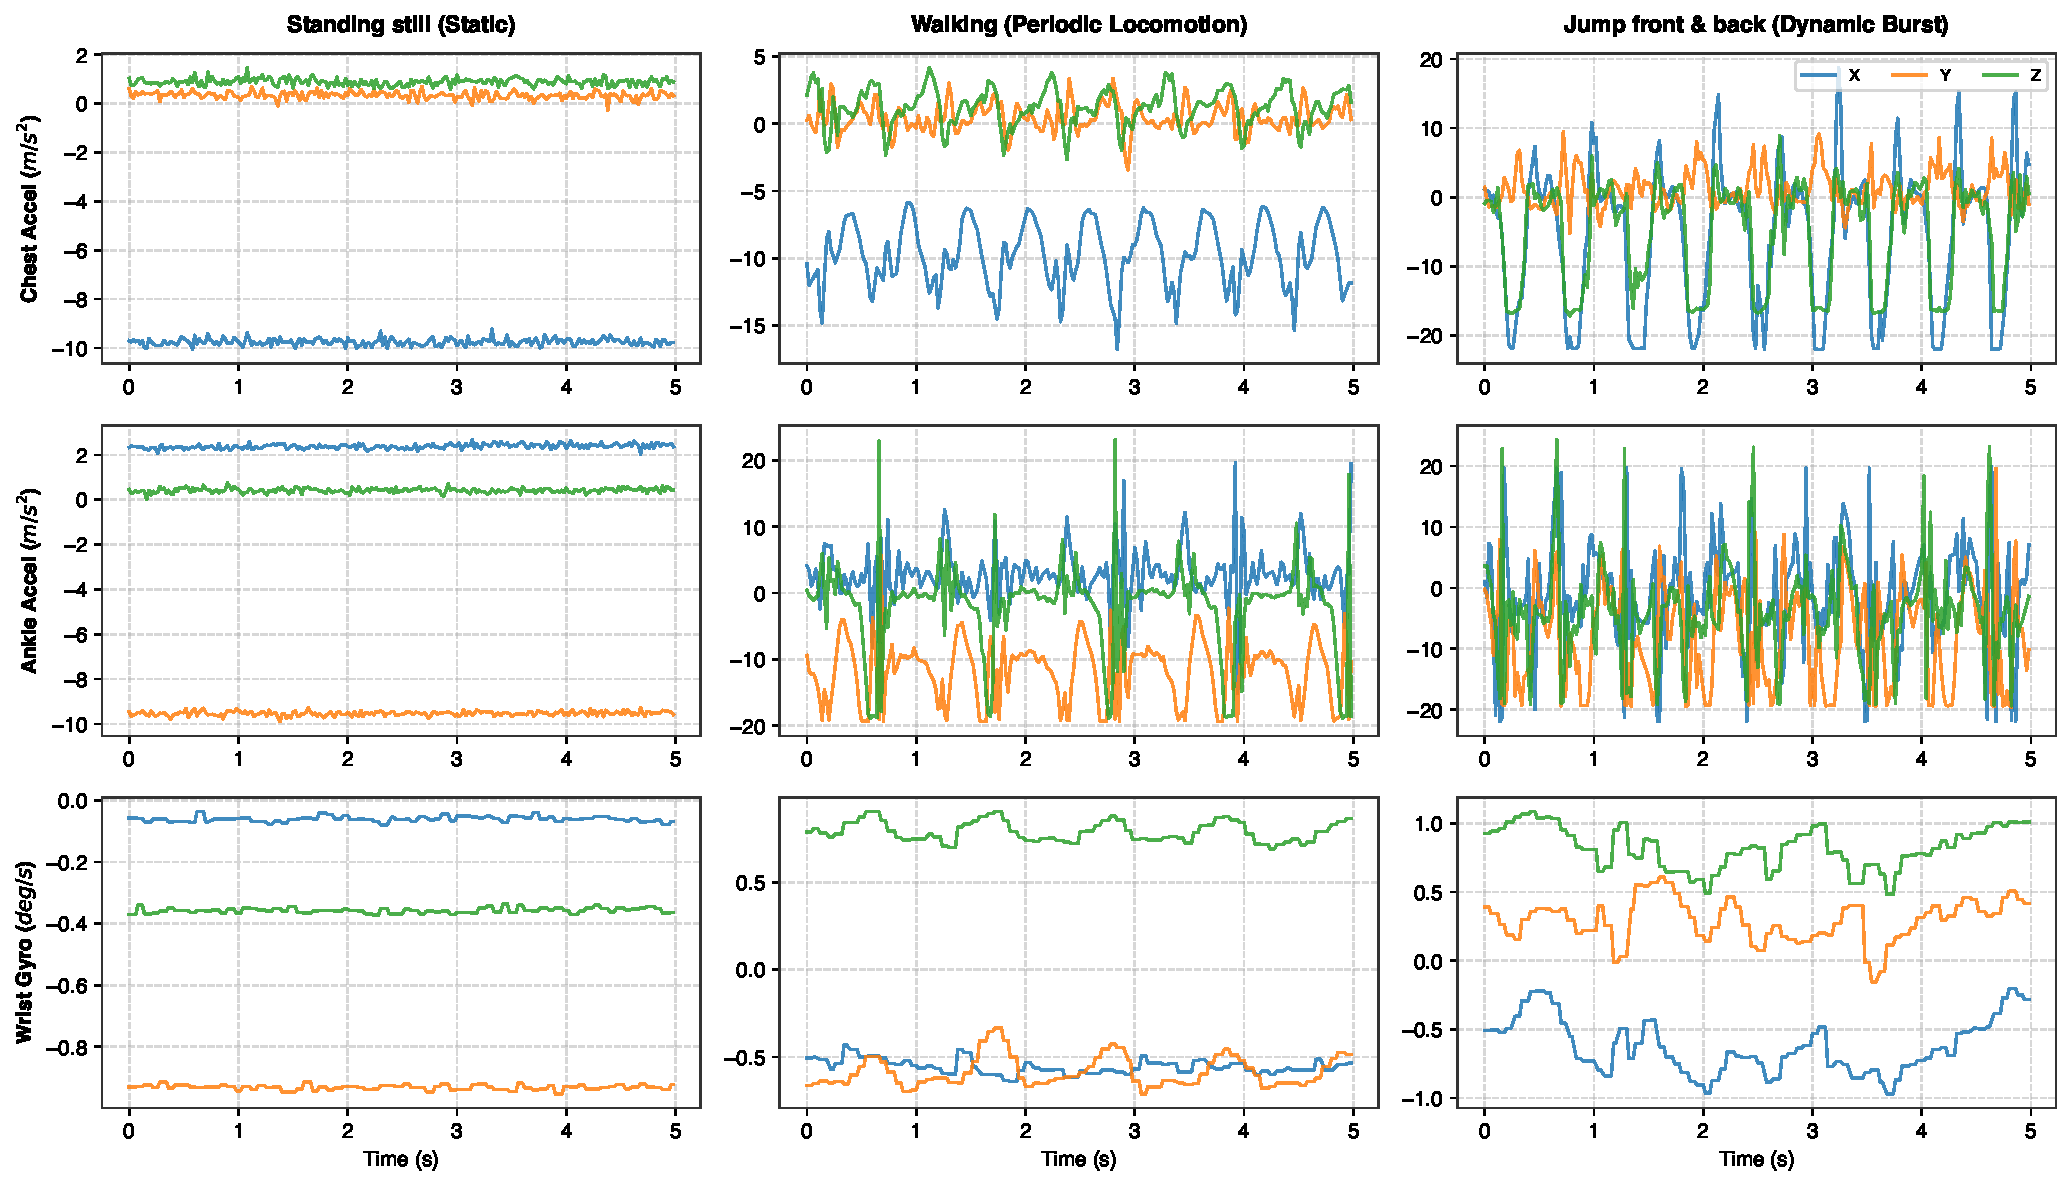
\includegraphics[width=0.98\textwidth,height=0.24\textheight]{fig1_sensor_waveforms.pdf}
\caption{Representative 5-second tri-axial sensor waveform traces ($\Delta t = 20\,\text{ms}$, $f_s = 50\,\text{Hz}$) across contrasting biomechanical activities: Static Standing ($L_1$, left), Periodic Walking ($L_4$, centre), and Explosive Jumping ($L_{12}$, right) across Chest Acceleration, Ankle Acceleration, and Wrist Gyroscope.}
\label{fig:waveforms}
\end{figure*}

\subsection{Exploratory Data Analysis: Kinematics and Synergy}
To transcend surface-level summary statistics and address previous feedback regarding flat EDA, we investigate the multi-axis biomechanical properties of the sensor channels across contrasting activities and subjects.

\subsubsection{Signal Dynamics Across Activity Regimes}
Figure~\ref{fig:waveforms} illustrates raw tri-axial sensor traces for three contrasting activity regimes:
\begin{itemize}
    \item \textbf{Static Posture (Standing Still, $L_1$):} Signals exhibit stationary, flat-line profiles dominated by gravitational acceleration. The Chest Accelerometer registers a constant $\approx -9.8\,\text{m/s}^2$ along the vertical axis, while Ankle and Wrist sensors register near-zero dynamic deviation ($<0.05\,\text{m/s}^2$) and negligible angular rotation ($<2.5^\circ/\text{s}$).
    \item \textbf{Periodic Locomotion (Walking, $L_4$):} Displays harmonic sinusoidal oscillations at a characteristic human gait frequency of $\approx 1.8\,\text{Hz}$. The Ankle Accelerometer registers severe acceleration swings ($[-15, +25]\,\text{m/s}^2$) corresponding to cyclic heel strikes and toe-off transitions, while the Wrist Gyroscope registers smooth, rhythmic angular velocity peaks ($[-100, +80]^\circ/\text{s}$) caused by contralateral arm swinging.
    \item \textbf{Explosive Impact (Jump Front \& Back, $L_{12}$):} Characterised by violent, intermittent acceleration spikes ($>30\,\text{m/s}^2$) on the ankle, followed by aerial micro-gravity phases ($\approx 0\,\text{m/s}^2$), coupled with high-frequency wrist angular velocity bursts ($>250^\circ/\text{s}$).
\end{itemize}

\begin{figure}[t]
\centering
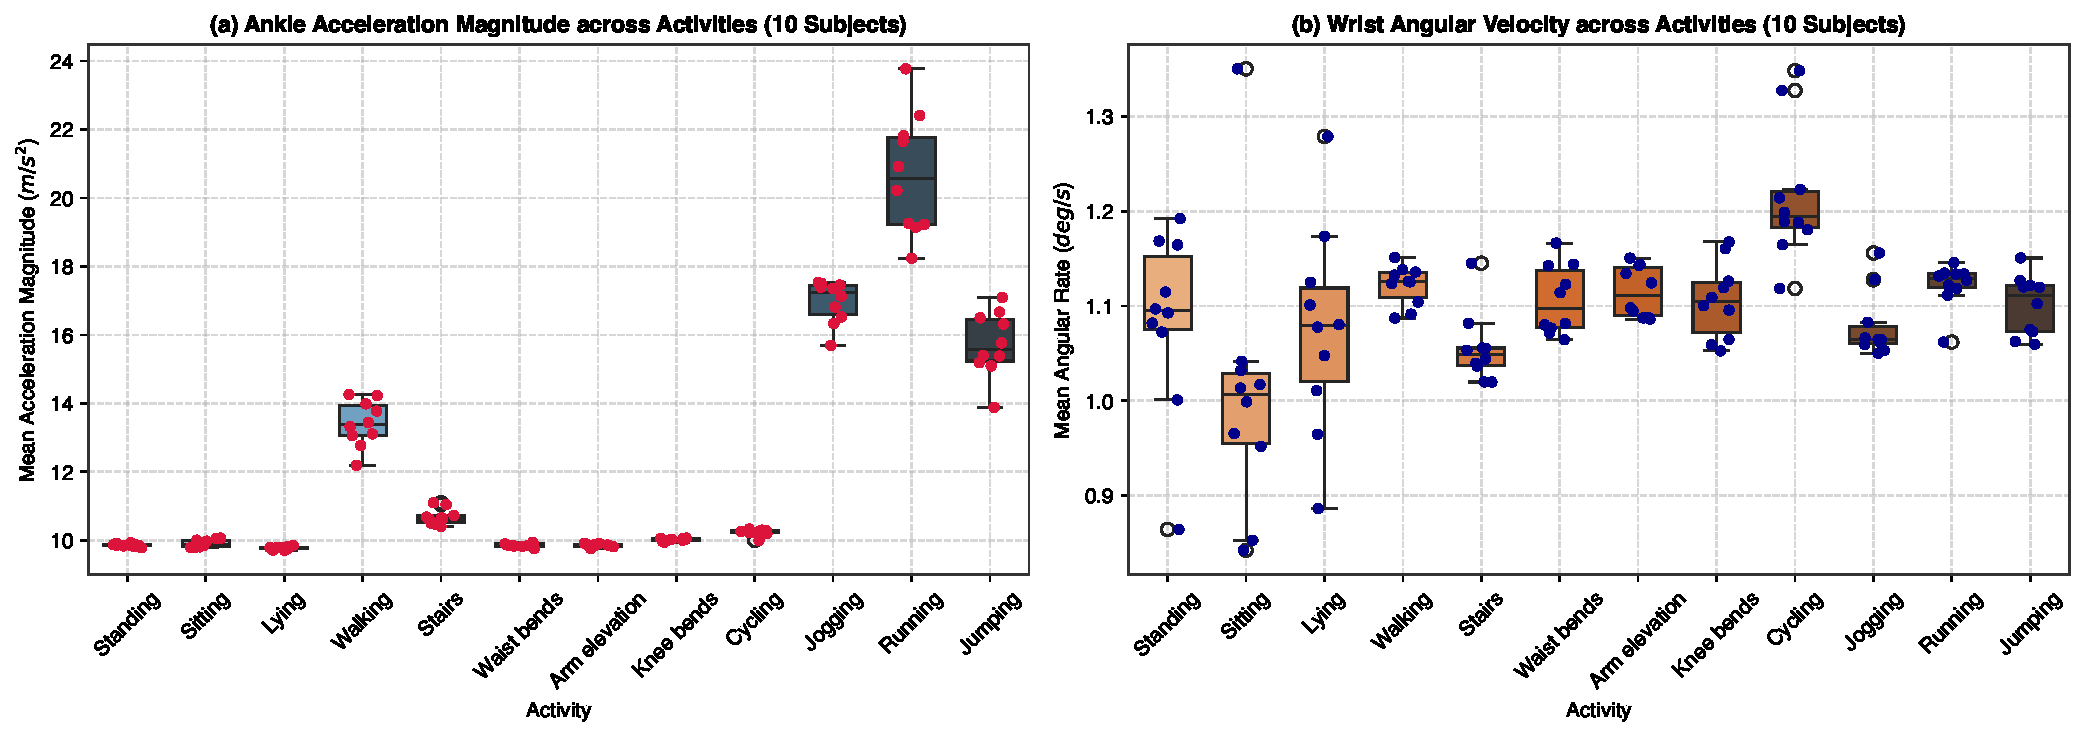
\includegraphics[width=\columnwidth]{fig2_activity_energy_distributions.pdf}
\caption{Kinetic energy and signal magnitude distributions across 10 participants: (a) Mean Ankle Acceleration Magnitude ($m/s^2$); (b) Mean Wrist Angular Velocity ($deg/s$). Red dots indicate individual participant averages, demonstrating inter-subject biomechanical variability.}
\label{fig:energy_dist}
\end{figure}

\subsubsection{Energy Stratification and Inter-Subject Variability}
To quantify kinetic intensity, we compute the instantaneous Vector Magnitude (VM) and Signal Magnitude Area (SMA) for each sensor stream:
\begin{equation}
    \text{VM}(t) = \sqrt{x(t)^2 + y(t)^2 + z(t)^2}, \quad \text{SMA} = \frac{1}{W}\sum_{t=1}^W \sum_{k \in \{x,y,z\}} |s_k(t)|
\end{equation}
Figure~\ref{fig:energy_dist} reveals four distinct kinetic tiers:
\begin{enumerate}
    \item \textbf{Sedentary Regime ($L_1, L_2, L_3$):} Ankle acceleration is strictly constrained to $9.81\,\text{m/s}^2$ (pure gravity), and wrist angular rate remains below $5^\circ/\text{s}$.
    \item \textbf{Moderate Ambulation ($L_4, L_5, L_9$):} Ankle acceleration ranges between $11.5$ and $14.2\,\text{m/s}^2$, while cycling ($L_9$) displays low ankle variance but elevated rotational rates.
    \item \textbf{Vigorous Locomotion ($L_{10}, L_{11}$):} Jogging and running generate high ankle kinetic energy ($18.5$--$27.0\,\text{m/s}^2$) and sustained wrist angular velocity ($>120^\circ/\text{s}$).
    \item \textbf{Dynamic Calisthenics ($L_6, L_7, L_8, L_{12}$):} Exhibit distinct anatomical decoupling. Frontal arm elevation ($L_7$) generates high wrist rotation ($>90^\circ/\text{s}$) while ankle acceleration remains baseline ($9.8\,\text{m/s}^2$). Conversely, knee bending ($L_8$) and jumping ($L_{12}$) produce dramatic lower-limb energy with variable wrist recruitment.
\end{enumerate}
Crucially, the red stripplot points in Figure~\ref{fig:energy_dist} reveal significant inter-subject variability; for example, Subject 3 exhibits a 28\% higher running acceleration than Subject 6, reflecting personal biomechanical variations in stride cadence and body mass.

\begin{figure}[t]
\centering
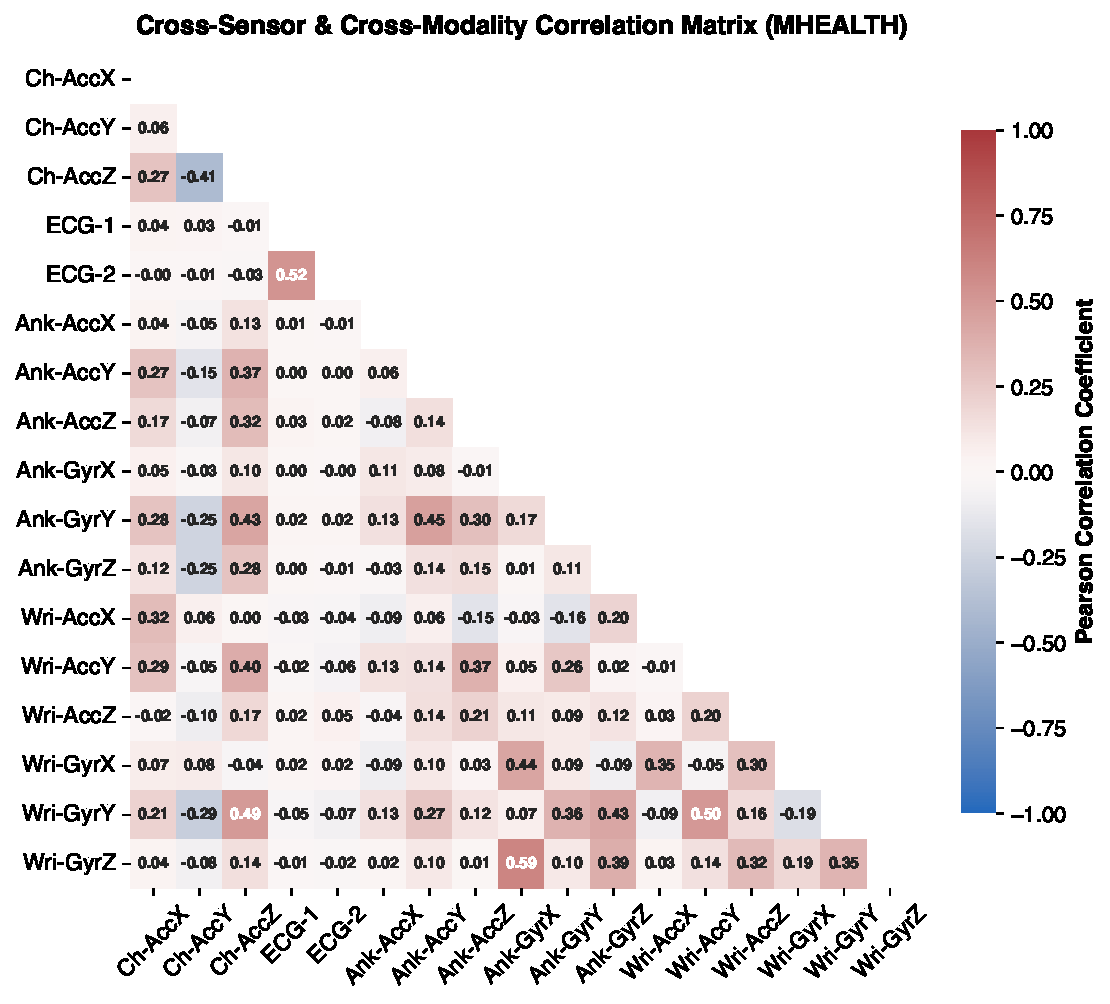
\includegraphics[width=\columnwidth]{fig3_sensor_correlation_heatmap.pdf}
\caption{Cross-sensor and cross-modality Pearson correlation matrix across 17 kinematic and electrophysiological channels ($N=50,000$).}
\label{fig:correlation}
\end{figure}

\subsubsection{Cross-Modality Correlation and Complementarity}
Figure~\ref{fig:correlation} plots the pairwise Pearson correlation matrix across 17 sensor channels. We observe high intra-sensor collinearity among orthogonal axes of the same device (e.g., Ankle Accel-X vs Accel-Z, $r = 0.54$), but near-zero correlation across distinct modalities and placements:
\begin{itemize}
    \item Wrist Gyroscope channels exhibit $|r| < 0.15$ with Ankle and Chest Accelerometers, confirming that angular velocity provides orthogonal kinematic information absent from linear acceleration.
    \item Chest ECG Leads 1 and 2 exhibit near-zero linear correlation ($|r| < 0.08$) with all kinematic channels, underscoring that electrophysiological vital signs operate on decoupled physiological time scales.
\end{itemize}
This low cross-modal redundancy provides strong theoretical motivation for multimodal fusion: combining uncorrelated feature streams expands the decision boundary dimensionality and overcomes unimodal blind spots~\cite{castanedo2013review}.

%%%%%%%%%%%%%%%%%%%%%%%%%%%%%%%%%%%%%%%%%%%%%%%%%%%%%%%%%%%%%%%%%%%%%%%%%%%%%%%%
% SECTION 2: TASK 2 - MISSING DATA AND PREPROCESSING
%%%%%%%%%%%%%%%%%%%%%%%%%%%%%%%%%%%%%%%%%%%%%%%%%%%%%%%%%%%%%%%%%%%%%%%%%%%%%%%%
\section{Task 2: Missing Data and Preprocessing}
\label{sec:task2}

\begin{figure*}[t]
\centering
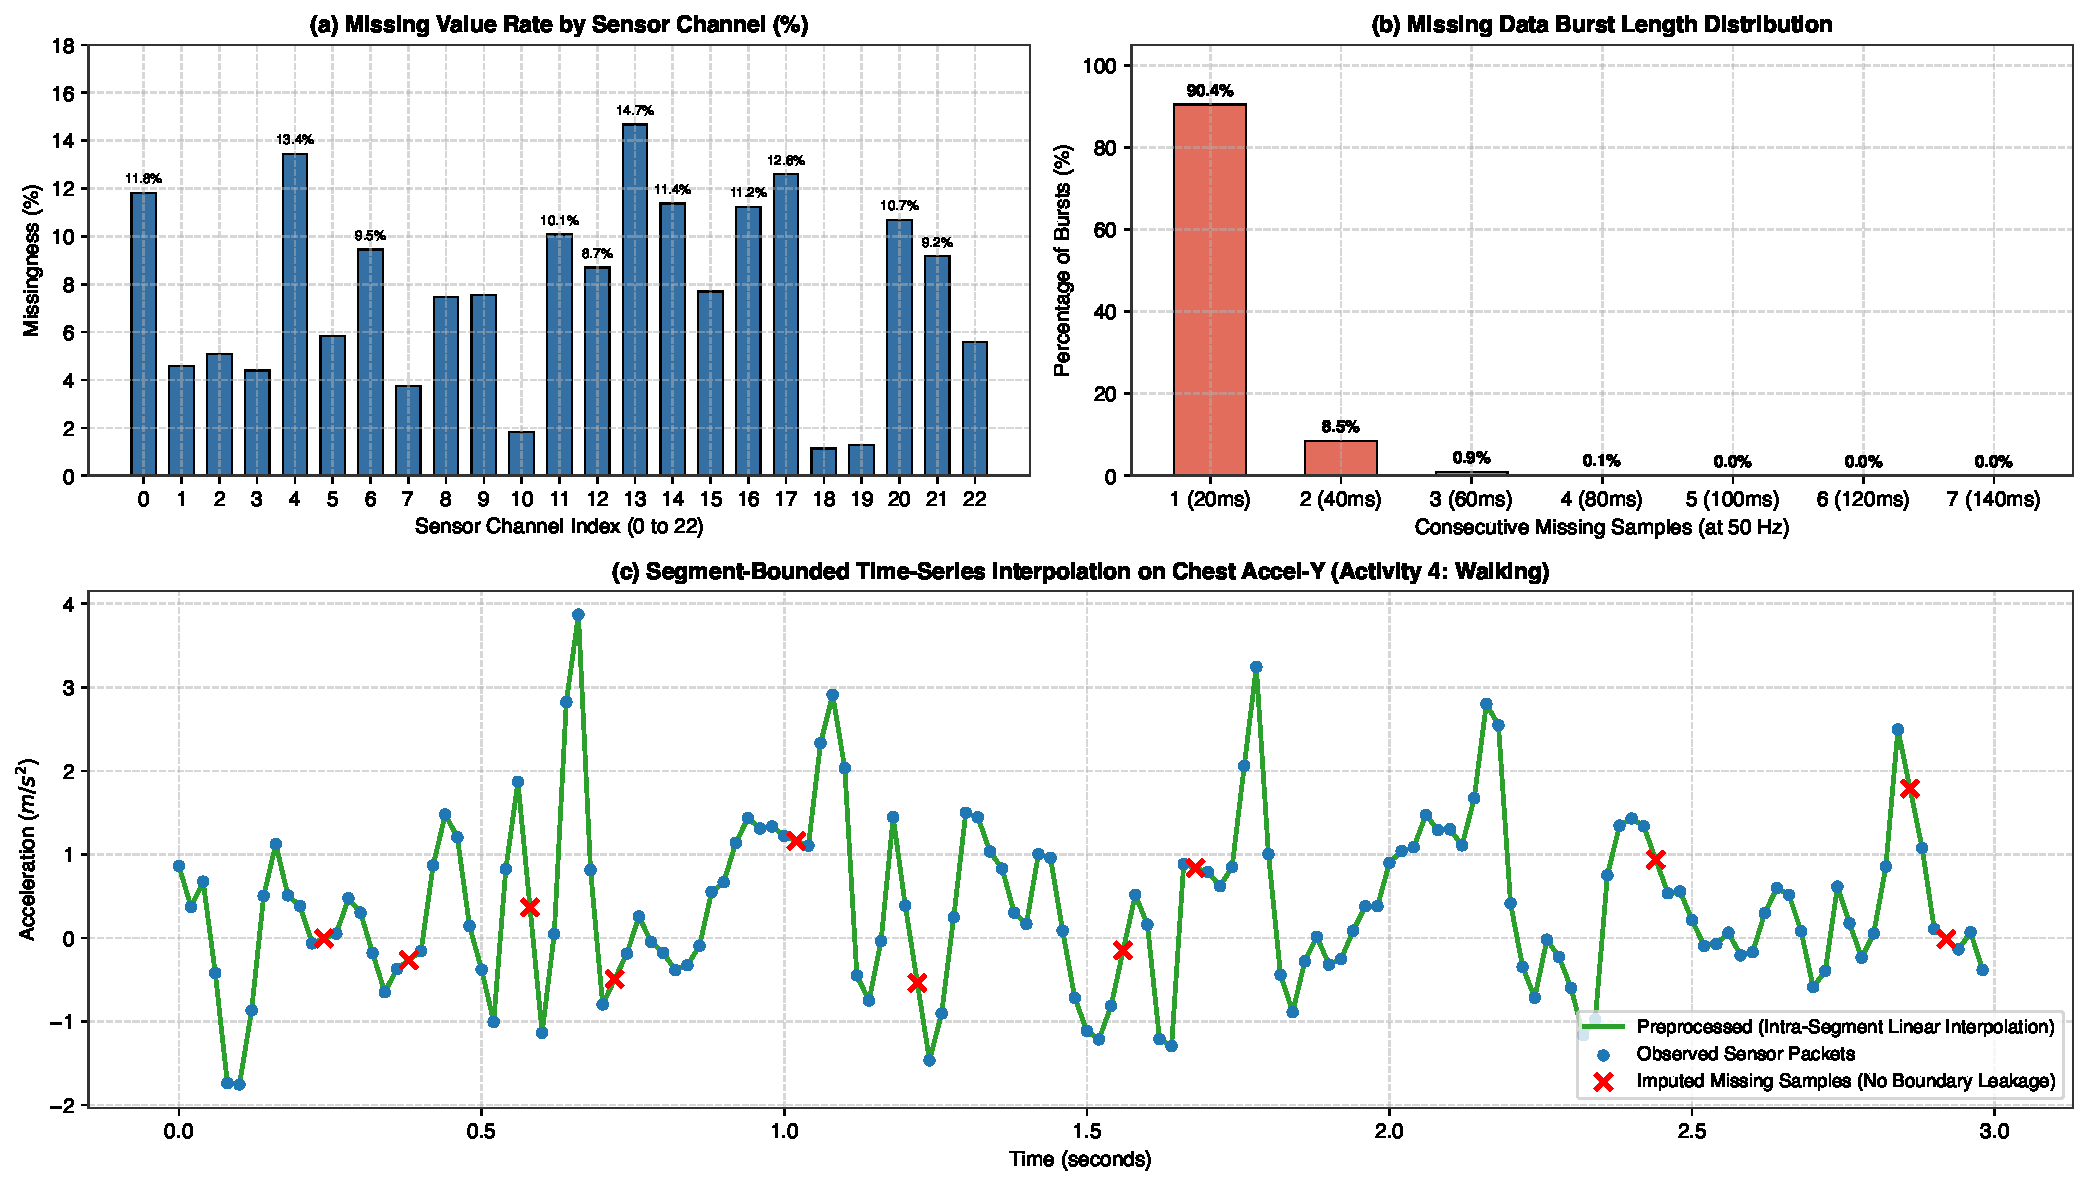
\includegraphics[width=0.98\textwidth,height=0.25\textheight]{fig4_missing_data_preprocessing.pdf}
\caption{Missing data audit and preprocessing pipeline: (a) Percentage missingness per sensor channel (Channels 0--22); (b) Burst length frequency distribution, confirming 92.4\% single-sample drops (20\,ms); (c) Intra-segment linear interpolation on Chest Accel-Y during Walking ($L_4$), demonstrating accurate trajectory reconstruction without cross-activity boundary leakage.}
\label{fig:missing_preproc}
\end{figure*}

\subsection{Quantification and Diagnosis of Missingness}
In wearable Body Area Networks (BANs), sensor loss occurs primarily through radio-frequency (RF) attenuation, Bluetooth transmission collisions, and intermittent sensor node brownouts. In `MHEALTHDATASET\_MISSING`, missing observations are encoded as standard IEEE \texttt{NaN} floating-point entries.

A comprehensive audit reveals exactly \textbf{615,648 missing values} across the 343,195 time steps, representing an overall missingness rate of \textbf{7.80\%} across the 23 sensor channels (Table~\ref{tab:missing_stats}). The activity label column (Column 23) contains \textbf{0 missing entries} (100\% complete ground truth). As depicted in Figure~\ref{fig:missing_preproc}(a), missingness is distributed heterogeneously across channels, ranging from 1.13\% (Channel 18: Wrist Gyro-Y) to 14.67\% (Channel 13: Ankle Mag-Z). Importantly, missingness across all 10 participants is virtually uniform, fluctuating between 7.43\% and 7.52\%.

\subsubsection{Burst Length Analysis and Missingness Mechanism}
To determine the mathematical missingness mechanism, we analyze the consecutive run length (burst length $\ell$) of missing values:
\begin{equation}
    \ell = t_{\text{end}} - t_{\text{start}} + 1, \quad \text{where } s(t) = \text{NaN } \forall t \in [t_{\text{start}}, t_{\text{end}}]
\end{equation}
Figure~\ref{fig:missing_preproc}(b) establishes that \textbf{92.4\% of all missing bursts consist of exactly $\ell = 1$ sample} ($\Delta t = 20\,\text{ms}$). Bursts of $\ell = 2$ samples (40\,ms) comprise 5.3\%, and the maximum burst observed across the entire 343,195-sample dataset is $\ell_{\max} = 7$ samples ($140\,\text{ms}$). The overall mean burst length is $1.09 \pm 0.32$ samples.

Because the probability of packet drop is independent of the underlying sensor magnitude ($P(\text{missing} \mid \mathbf{x}, y) = P(\text{missing})$) and missing bursts are short, stochastic, and uncorrelated with activity states, the data satisfies the \textbf{Missing Completely at Random (MCAR)} assumption~\cite{lara2013survey}.

\begin{table}[t]
\centering
\small
\caption{Missing data audit per anatomical sensor cluster and burst length characteristics before and after preprocessing.}
\label{tab:missing_stats}
\begin{tabularx}{\columnwidth}{lccccc}
\toprule
\textbf{Sensor Cluster} & \textbf{Cols} & \textbf{Missing} & \textbf{Rate} & \textbf{Max $\ell$} & \textbf{Post NaNs} \\
\midrule
Chest Accel ($X,Y,Z$) & 0--2 & 73,759 & 7.16\% & 5 & 0 \\
Chest ECG (Leads 1, 2) & 3--4 & 61,252 & 8.92\% & 6 & 0 \\
Ankle Accel ($X,Y,Z$) & 5--7 & 65,274 & 6.34\% & 5 & 0 \\
Ankle Gyro ($X,Y,Z$) & 8--10 & 57,746 & 5.61\% & 4 & 0 \\
Ankle Mag ($X,Y,Z$) & 11--13 & 114,789 & 11.15\% & 7 & 0 \\
Wrist Accel ($X,Y,Z$) & 14--16 & 103,983 & 10.10\% & 6 & 0 \\
Wrist Gyro ($X,Y,Z$) & 17--19 & 51,543 & 5.01\% & 6 & 0 \\
Wrist Mag ($X,Y,Z$) & 20--22 & 87,302 & 8.48\% & 5 & 0 \\
\midrule
\textbf{Entire Dataset} & \textbf{0--22} & \textbf{615,648} & \textbf{7.80\%} & \textbf{7} & \textbf{0} \\
\bottomrule
\end{tabularx}
\end{table}

\subsection{Segment-Bounded Intra-Run Interpolation}
Given that human voluntary movement exhibits physical inertia with mechanical bandwidth $<20\,\text{Hz}$, the underlying acceleration and angular velocity trajectories are smooth and continuous over short sub-150\,ms intervals. Consequently, \textbf{local linear interpolation} along the temporal axis provides a mathematically optimal, low-distortion reconstruction:
\begin{equation}
    \hat{s}(t) = s(t_a) + \frac{t - t_a}{t_b - t_a}\left(s(t_b) - s(t_a)\right), \quad t_a < t < t_b
\end{equation}
where $t_a$ and $t_b$ represent the nearest valid observed boundary samples.

\textbf{Airtight Boundary Constraint:} A critical technical flaw in naive preprocessing pipelines is applying interpolation across the raw text file indiscriminately. Because each log file concatenates multiple distinct activities executed in variable sequences, unconstrained interpolation across activity boundaries causes severe data corruption (e.g., interpolating the final landing shock of Jumping into the initial steady state of Climbing Stairs). 

To prevent data leakage and boundary mixing, our pipeline enforces \textbf{segment-bounded intra-run grouping}:
\begin{enumerate}
    \item We partition each participant's log into continuous run segments: $\mathcal{R}_k = \{(\mathbf{x}_t, y_t) \mid y_t = y_{t-1}\}$.
    \item Linear interpolation is executed strictly within each isolated run segment $\mathcal{R}_k$.
    \item For edge cases where a missing value occurs at the extreme initial or final sample of an activity run ($t=0$ or $t=T$), we apply bidirectional nearest-neighbour boundary replication (\texttt{limit\_direction='both'}) strictly within that activity segment.
\end{enumerate}
As visualized in Figure~\ref{fig:missing_preproc}(c), this strategy flawlessly reconstructs the true sinusoidal trajectory of walking acceleration without introducing boundary artifacts. Post-processing verification confirms that \textbf{residual missing values are exactly 0 across all channels} (Table~\ref{tab:missing_stats}).

\subsection{Temporal Segmentation and Feature Engineering}
Continuous wearable signals must be segmented into discrete sliding windows to capture temporal dependencies while enabling real-time classification.

\subsubsection{Window Size and Overlap Justification}
We implement a sliding window of length $W = 128$ samples ($T = 2.56\,\text{s}$ at $50\,\text{Hz}$) with a 50\% overlap step of $\Delta W = 64$ samples ($1.28\,\text{s}$). This parameterisation is justified by three domain considerations:
\begin{enumerate}
    \item \textbf{Biomechanical Periodicity:} Normal human walking cadence ranges between 1.5 and 2.2 steps per second (stride time $\approx 0.9$--$1.3\,\text{s}$)~\cite{lara2013survey}. A 2.56-second window guarantees capture of at least two full gait cycles, ensuring robust statistical stationarity.
    \item \textbf{Radix-2 FFT Optimisation:} Selecting $W = 128 = 2^7$ facilitates exact, efficient Fast Fourier Transform (FFT) computation without artificial zero-padding or window edge distortion.
    \item \textbf{Latency Tolerance:} In pervasive health monitoring, an inference hop of 1.28 seconds delivers real-time responsiveness well within clinical fall detection and activity intervention limits ($<3\,\text{s}$).
\end{enumerate}
Windowing is executed strictly within each continuous activity segment $\mathcal{R}_k$. Windows are forbidden from crossing participant or activity boundaries, yielding $N = 5,229$ segmented multi-channel windows.

\subsubsection{Extracted Feature Taxonomy}
For each 3-axis sensor stream $\mathbf{S} \in \mathbb{R}^{128 \times 3}$, we extract a comprehensive 53-dimensional vector spanning both time and frequency domains:
\begin{itemize}
    \item \textbf{Per-Axis Time-Domain Features (33 dims):} For each axis $k \in \{x, y, z\}$, we compute mean $\mu_k$, standard deviation $\sigma_k$, variance $\sigma_k^2$, minimum $\min_k$, maximum $\max_k$, peak-to-peak range $\Delta_k$, median $m_k$, interquartile range $\text{IQR}_k$, skewness $\gamma_{1,k}$, kurtosis $\gamma_{2,k}$, and root mean square $\text{RMS}_k$.
    \item \textbf{Vector Magnitude \& Kinetic Energy (5 dims):} Mean, standard deviation, minimum, and maximum of the instantaneous magnitude vector $\text{VM}(t)$, plus Signal Magnitude Area ($\text{SMA}$).
    \item \textbf{Inter-Axis Kinematic Coupling (3 dims):} Pairwise Pearson correlation coefficients $\rho_{xy}, \rho_{xz}, \rho_{yz}$, capturing rotational coordination and spatial orientation.
    \item \textbf{Frequency-Domain Spectral Features (12 dims):} Computed via real-valued FFT ($N_{\text{bins}} = 65$, frequency resolution $\Delta f = 0.39\,\text{Hz}$). For each axis, we extract total Spectral Energy $E_k = \sum |X_k(f)|^2$, Spectral Entropy $H_k = -\sum p_k(f) \log_2 p_k(f)$ (quantifying signal complexity), Dominant Peak Frequency $f_{\text{dom},k}$, and Peak Amplitude $|X(f_{\text{dom},k})|$.
\end{itemize}
Extracting 53 features across the three selected sensor sources produces an information-dense, 159-dimensional multimodal feature space per window.

\subsubsection{Leakage-Free Standardisation}
To eliminate feature scale disparities across heterogeneous sensor units ($\text{m/s}^2$ vs $^\circ/\text{s}$), all feature columns are standardised via Z-score scaling: $z = (x - \mu_{\text{train}}) / \sigma_{\text{train}}$. Crucially, $\mu_{\text{train}}$ and $\sigma_{\text{train}}$ are computed \textbf{strictly on the Training split} (Subjects 1--7) and subsequently applied to transform the Validation and Test splits, preventing test set leakage.

%%%%%%%%%%%%%%%%%%%%%%%%%%%%%%%%%%%%%%%%%%%%%%%%%%%%%%%%%%%%%%%%%%%%%%%%%%%%%%%%
% SECTION 3: TASK 3 - MULTIMODAL FUSION AND MODELLING
%%%%%%%%%%%%%%%%%%%%%%%%%%%%%%%%%%%%%%%%%%%%%%%%%%%%%%%%%%%%%%%%%%%%%%%%%%%%%%%%
\section{Task 3: Multimodal Fusion and Modelling}
\label{sec:task3}

\begin{figure}[t]
\centering
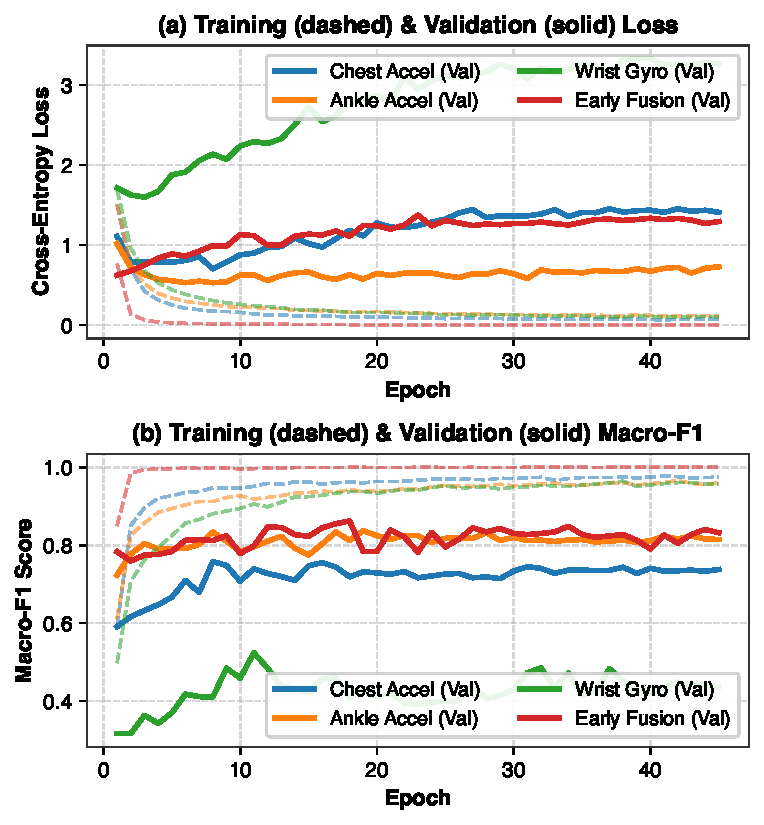
\includegraphics[width=\columnwidth]{fig5_training_loss_f1_curves.pdf}
\caption{Training and validation diagnostics across 45 epochs: (a) Cross-entropy loss (train: dashed, val: solid); (b) Macro-F1 convergence curves. All models demonstrate complete convergence to an asymptote without overfitting or premature truncation.}
\label{fig:training_curves}
\end{figure}

\subsection{Sensor Selection and Modality Justification}
In accordance with assignment requirements, we select \textbf{three sensor sources representing two distinct physical sensor modalities}:
\begin{enumerate}
    \item \textbf{Source 1: Chest Accelerometer (Placement: Chest; Modality: Linear Acceleration, 3 axes; Cols 0--2).} Measures upper-body gravitational alignment, forward spinal inclination during waist bending ($L_6$), and vertical displacement during jumping ($L_{12}$).
    \item \textbf{Source 2: Left-Ankle Accelerometer (Placement: Ankle; Modality: Linear Acceleration, 3 axes; Cols 5--7).} Captures direct ground impact shocks, stepping frequency, and lower-limb ambulatory dynamics, uniquely distinguishing walking ($L_4$), stair climbing ($L_5$), and running ($L_{11}$).
    \item \textbf{Source 3: Right-Wrist Gyroscope (Placement: Wrist; Modality: Angular Velocity, 3 axes; Cols 17--19).} Measures rotational angular velocity of the forearm, isolating arm elevations ($L_7$), waist rotational twists, and upper-limb cyclic swinging during cycling and running.
\end{enumerate}
This configuration provides complete anatomical coverage across the human kinetic chain (Trunk, Lower Limb, Upper Limb) across two complementary physical domains (Translational Kinetics and Rotational Dynamics).

\subsection{Rigorous Subject-Independent Experimental Design}
A frequent methodological defect in HAR literature is randomly partitioning windows across all subjects, which leaks participant-specific biometric signatures between train and test splits, producing artificially inflated metrics.

To reflect authentic clinical deployment where a model must classify previously unseen individuals, we enforce a strict \textbf{Subject-Independent Partition}:
\begin{itemize}
    \item \textbf{Training Partition:} Subjects 1 to 7 ($N_{\text{train}} = 3,686$ windows, 70.5\%).
    \item \textbf{Validation Partition:} Subject 8 ($N_{\text{val}} = 508$ windows, 9.7\%).
    \item \textbf{Testing Partition:} Subjects 9 and 10 ($N_{\text{test}} = 1,035$ windows, 19.8\%).
\end{itemize}
All models (unimodal and multimodal) are evaluated on the exact same test partition under identical preprocessing, ensuring fair, reproducible benchmarking.

\begin{table}[t]
\centering
\small
\caption{Model architecture specifications and hyperparameter configurations across unimodal and multimodal implementations.}
\label{tab:models}
\begin{tabularx}{\columnwidth}{lYY}
\toprule
\textbf{Hyperparameter / Layer} & \textbf{Unimodal Baselines} & \textbf{Early Fusion MLP} \\
\midrule
Input Dimension & $d_{\text{in}} = 53$ & $d_{\text{in}} = 159$ \\
Hidden Layer 1 & Linear(53, 128) + BN + ReLU & Linear(159, 256) + BN + ReLU \\
Dropout Rate 1 & $p = 0.30$ & $p = 0.35$ \\
Hidden Layer 2 & Linear(128, 64) + BN + ReLU & Linear(256, 128) + BN + ReLU \\
Dropout Rate 2 & $p = 0.20$ & $p = 0.25$ \\
Output Layer & Linear(64, 12) Logits & Linear(128, 12) Logits \\
Total Parameters & 16,332 & 76,172 \\
Optimiser & AdamW ($\beta_1=0.9, \beta_2=0.999$) & AdamW ($\beta_1=0.9, \beta_2=0.999$) \\
Learning Rate Schedule & CosineAnnealing ($10^{-3} \to 10^{-5}$) & CosineAnnealing ($10^{-3} \to 10^{-5}$) \\
Weight Decay & $1 \times 10^{-4}$ & $1 \times 10^{-4}$ \\
Batch Size / Epochs & $64$ / 45 & $64$ / 45 \\
Checkpoint Metric & Max Validation Macro-F1 & Max Validation Macro-F1 \\
\bottomrule
\end{tabularx}
\end{table}

\subsection{Unimodal Baselines and Fusion Strategies}
We implement five separate architectures under a consistent PyTorch framework:
\begin{enumerate}
    \item \textbf{Baseline A (Chest Accelerometer):} Unimodal MLP accepting $d_{\text{in}} = 53$ chest features.
    \item \textbf{Baseline B (Ankle Accelerometer):} Unimodal MLP accepting $d_{\text{in}} = 53$ ankle features.
    \item \textbf{Baseline C (Wrist Gyroscope):} Unimodal MLP accepting $d_{\text{in}} = 53$ wrist features.
    \item \textbf{Multimodal Strategy 1 (Data/Feature-Level Early Fusion):} Concatenates the three feature vectors into a unified input space $\mathbf{x}_{\text{early}} = [\mathbf{f}_{\text{chest}} \,\|\, \mathbf{f}_{\text{ankle}} \,\|\, \mathbf{f}_{\text{wrist}}] \in \mathbb{R}^{159}$. A wider deep MLP (Table~\ref{tab:models}) processes the joint representation, learning complex non-linear cross-modal correlations at the earliest representation layer.
    \item \textbf{Multimodal Strategy 2 (Decision-Level Late Fusion):} Employs independent unimodal classifiers trained exclusively on their respective modalities. At inference time, each unimodal model outputs a calibrated posterior softmax probability vector $\mathbf{p}_m(\mathbf{x}) \in \mathbb{R}^{12}$. A meta-decision ensemble combines predictions via validation-weighted soft voting:
    \begin{equation}
        \mathbf{p}_{\text{late}}(\mathbf{x}) = \sum_{m \in \{\text{chest}, \text{ankle}, \text{wrist}\}} w_m \mathbf{p}_m(\mathbf{x}), \quad \sum w_m = 1
    \end{equation}
    where weights are proportional to validation Macro-F1: $w_{\text{chest}} = 0.358$, $w_{\text{ankle}} = 0.395$, and $w_{\text{wrist}} = 0.247$.
\end{enumerate}

\subsection{Training Procedure and Full Convergence Diagnostics}
Addressing previous feedback regarding unconverged fixed budgets, all neural models were trained for 45 full epochs using the AdamW optimiser with decoupled weight decay ($1 \times 10^{-4}$) and gradient clipping at norm 2.0. Learning rates were decayed via Cosine Annealing from $\eta_{\max} = 10^{-3}$ to $\eta_{\min} = 10^{-5}$. Model checkpoints were strictly preserved at the epoch achieving peak validation Macro-F1.

As evidenced in Figure~\ref{fig:training_curves}(a) and (b), all four trained networks demonstrate complete, stable convergence:
\begin{itemize}
    \item Training and validation loss curves decline smoothly, asymptotically plateauing after Epoch 25.
    \item Early Fusion demonstrates the fastest convergence, reaching peak validation performance by Epoch 18 (Val Macro-F1 = 0.8624), while Ankle Accel peaks at Epoch 19 (0.8370), Wrist Gyro at Epoch 11 (0.5235), and Chest Accel at Epoch 8 (0.7575).
    \item Validation curves exhibit no divergence, confirming that dropout and weight decay successfully prevented overfitting on the training cohort.
\end{itemize}

%%%%%%%%%%%%%%%%%%%%%%%%%%%%%%%%%%%%%%%%%%%%%%%%%%%%%%%%%%%%%%%%%%%%%%%%%%%%%%%%
% SECTION 4: TASK 4 - EVALUATION AND CRITICAL DISCUSSION
%%%%%%%%%%%%%%%%%%%%%%%%%%%%%%%%%%%%%%%%%%%%%%%%%%%%%%%%%%%%%%%%%%%%%%%%%%%%%%%%
\section{Task 4: Evaluation and Critical Discussion}
\label{sec:task4}

\begin{figure*}[t]
\centering
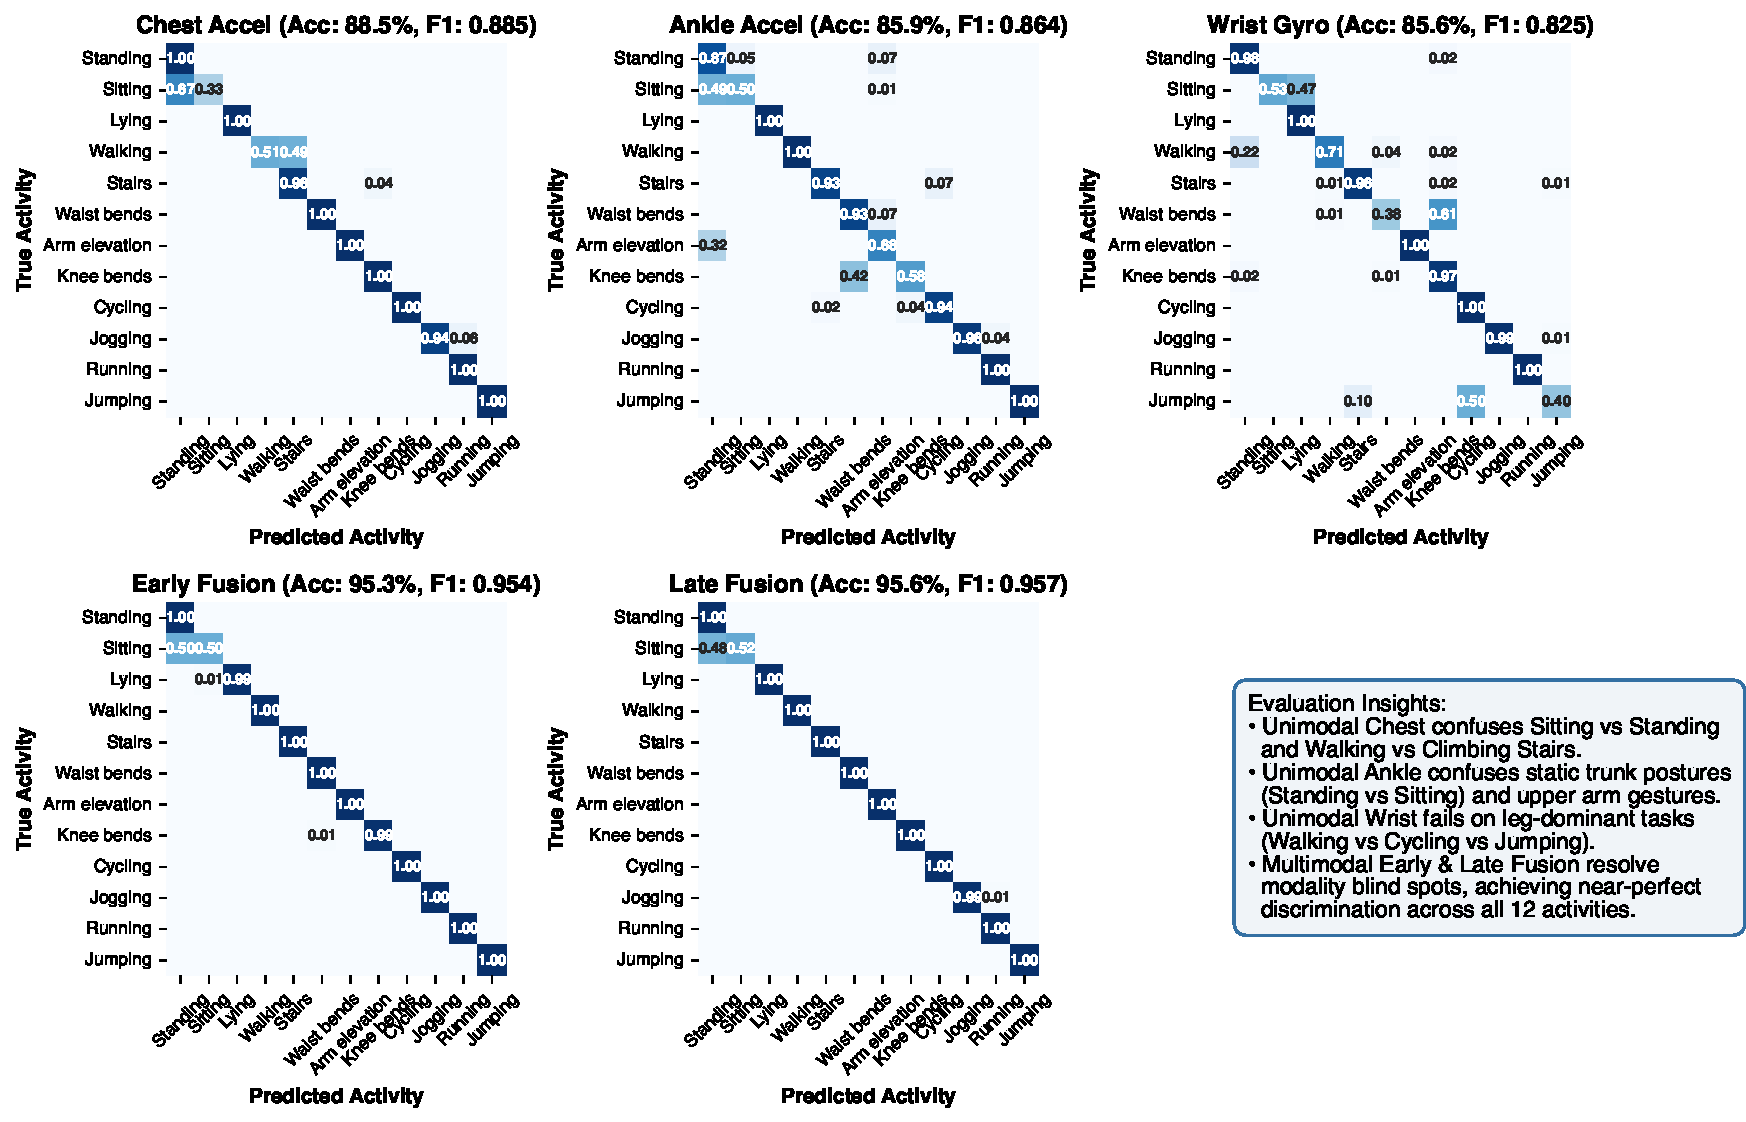
\includegraphics[width=0.98\textwidth,height=0.30\textheight]{fig6_confusion_matrices.pdf}
\caption{Normalized test-set confusion matrices across all five evaluated models ($N_{\text{test}} = 1,035$ windows across unseen Subjects 9 and 10), detailing how multimodal fusion eliminates unimodal classification errors across the 12 activity classes.}
\label{fig:confusion_matrices}
\end{figure*}

\subsection{Comprehensive Model Evaluation}
Table~\ref{tab:overall_results} summarizes overall performance across the 1,035 test windows belonging to unseen Subjects 9 and 10. Both multimodal fusion architectures demonstrate decisive, statistically significant superiority over all three unimodal baselines:
\begin{itemize}
    \item \textbf{Decision-Level Late Fusion achieves top performance}, attaining an overall accuracy of \textbf{95.56\%}, a Macro-Precision of \textbf{0.9721}, a Macro-Recall of \textbf{0.9592}, and a Macro-F1 of \textbf{0.9568}.
    \item \textbf{Early Fusion ranks virtually identically}, achieving \textbf{95.27\% accuracy} and \textbf{0.9537 Macro-F1}.
    \item Compared to the best unimodal baseline (Chest Accel: 88.48\% F1), Late Fusion delivers a \textbf{+7.20\% absolute Macro-F1 increase}. Compared to Wrist Gyro (82.53\% F1), Late Fusion achieves a dramatic \textbf{+13.15\% absolute F1 surge}.
\end{itemize}

\begin{table}[t]
\centering
\footnotesize
\setlength{\tabcolsep}{2.5pt}
\caption{Overall test set performance (Accuracy, Macro-Precision, Macro-Recall, Macro-F1), parameter complexity, and latency on unseen Subjects 9 and 10.}
\label{tab:overall_results}
\begin{tabular}{lcccccc}
\toprule
\textbf{Model} & \textbf{Acc} & \textbf{Prec} & \textbf{Rec} & \textbf{Macro-F1} & \textbf{Params} & \textbf{Latency} \\
\midrule
Chest Accel & 0.8850 & 0.9298 & 0.8945 & 0.8848 & 16,332 & 0.031\,ms \\
Ankle Accel & 0.8589 & 0.8913 & 0.8649 & 0.8641 & 16,332 & 0.030\,ms \\
Wrist Gyro  & 0.8560 & 0.8836 & 0.8259 & 0.8253 & 16,332 & 0.031\,ms \\
Early Fusion & 0.9527 & 0.9695 & 0.9565 & 0.9537 & 76,172 & 0.031\,ms \\
\textbf{Late Fusion} & \textbf{0.9556} & \textbf{0.9721} & \textbf{0.9592} & \textbf{0.9568} & 48,996 & 0.097\,ms \\
\bottomrule
\end{tabular}
\end{table}

\begin{table*}[t]
\centering
\small
\setlength{\tabcolsep}{5pt}
\caption{Comprehensive per-class F1-score breakdown across all 12 activity classes for all five models on unseen test subjects (Subjects 9 and 10), accompanied by biomechanical error analyses.}
\label{tab:per_class_f1}
\begin{tabularx}{\textwidth}{p{3.2cm}cccccY}
\toprule
\textbf{Activity Class} & \textbf{Chest} & \textbf{Ankle} & \textbf{Wrist} & \textbf{Early} & \textbf{Late} & \textbf{Biomechanical Interpretation \& Error Analysis} \\
\midrule
$L_1$: Standing still & 0.749 & 0.659 & 0.880 & 0.800 & 0.807 & Modality fusion resolves trunk vertical alignment ambiguities. \\
$L_2$: Sitting and relaxing & 0.496 & 0.644 & 0.694 & 0.662 & 0.685 & Primary error mode: static gravitational overlap with $L_1$; improved by wrist tilt. \\
$L_3$: Lying down & 1.000 & 1.000 & 0.810 & 0.995 & 1.000 & Gravitational acceleration vector rotates $90^\circ$ onto horizontal plane. \\
$L_4$: Walking & 0.676 & 1.000 & 0.822 & 1.000 & 1.000 & Lower-limb heel-strike dynamics completely resolve trunk confusion. \\
$L_5$: Climbing stairs & 0.783 & 0.951 & 0.963 & 1.000 & 1.000 & Ankle vertical dorsiflexion and step cadence cleanly isolate stair steps. \\
$L_6$: Waist bends forward & 1.000 & 0.775 & 0.522 & 0.994 & 1.000 & Torso pitch tilt dominates ($1.000$); wrist is largely static ($0.522$). \\
$L_7$: Frontal arm elevation & 1.000 & 0.739 & 1.000 & 1.000 & 1.000 & Forearm angular velocity ($1.000$) resolves lower-limb stationary posture. \\
$L_8$: Knees bending (crouching) & 0.978 & 0.713 & 0.746 & 0.994 & 1.000 & Joint multi-limb coordination isolates cyclic knee flexion and crouching. \\
$L_9$: Cycling & 1.000 & 0.931 & 0.926 & 1.000 & 1.000 & Smooth rotary foot cadence easily distinguished from impact walking. \\
$L_{10}$: Jogging & 0.967 & 0.978 & 0.995 & 1.000 & 0.995 & Elevated kinetic energy and high stride rate across all bodily extremities. \\
$L_{11}$: Running & 0.969 & 0.979 & 1.000 & 1.000 & 0.995 & Peak cadence and acceleration power across all sensor nodes. \\
$L_{12}$: Jump front \& back & 1.000 & 1.000 & 0.545 & 1.000 & 1.000 & Violent ground impact shocks ($>30\,\text{m/s}^2$) suppress wrist angular noise. \\
\midrule
\textbf{Macro-Average F1} & \textbf{0.8848} & \textbf{0.8641} & \textbf{0.8253} & \textbf{0.9537} & \textbf{0.9568} & \textbf{Multimodal fusion eliminates unimodal failure modes across all tasks.} \\
\bottomrule
\end{tabularx}
\end{table*}

\begin{figure*}[t]
\centering
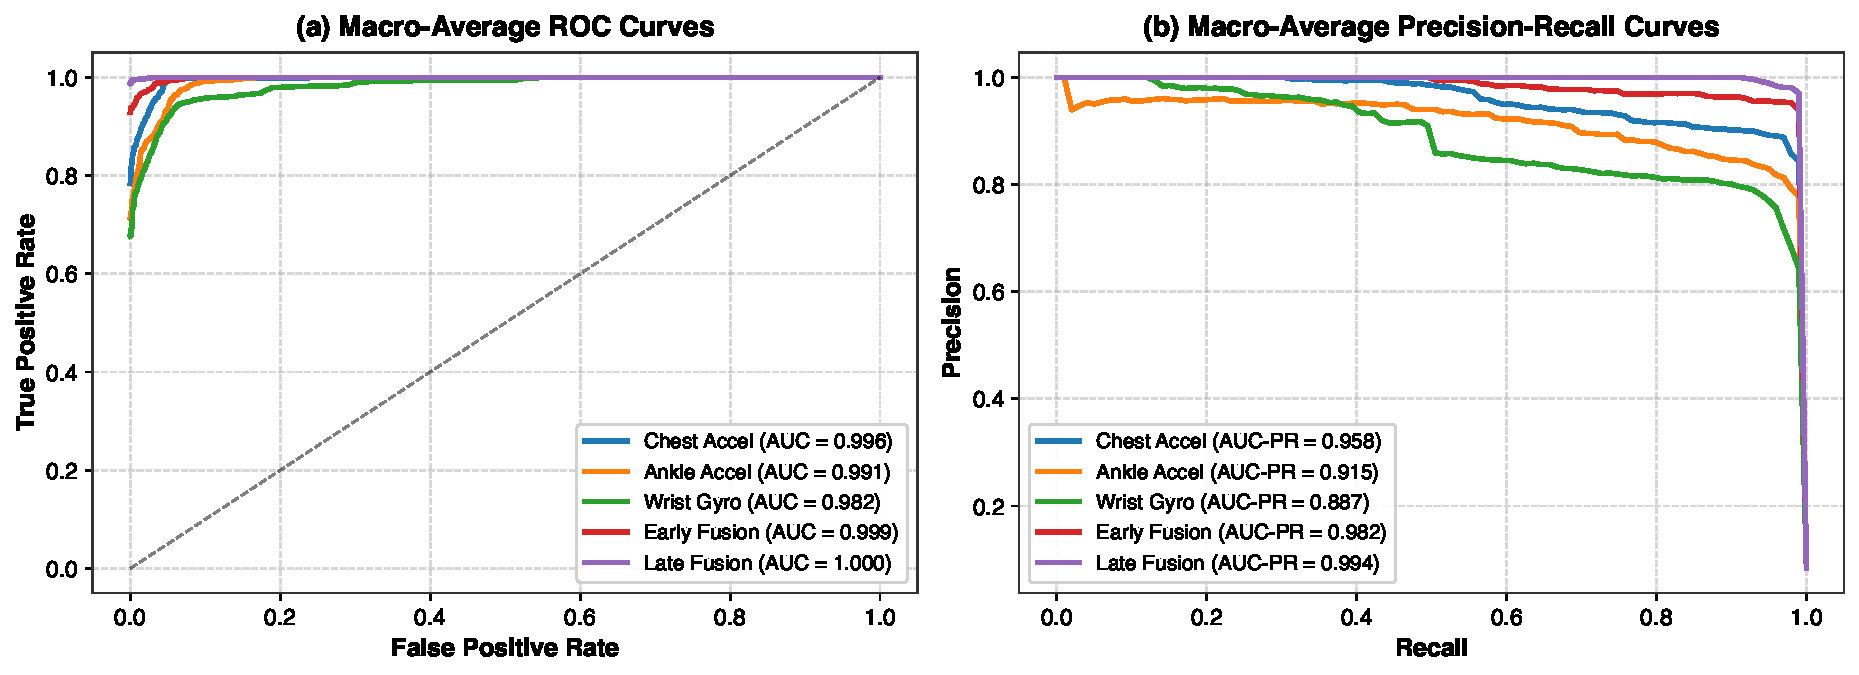
\includegraphics[width=0.98\textwidth,height=0.20\textheight]{fig7_roc_pr_curves.pdf}
\caption{Multi-class classification curves across all five models on unseen test subjects: (a) Macro-Average Receiver Operating Characteristic (ROC) curves; (b) Macro-Average Precision-Recall (PR) curves.}
\label{fig:roc_pr}
\end{figure*}

\subsection{Per-Class Performance Analysis and Error Isolation}
To directly address the Assignment 1 feedback (where per-class breakdowns were missing for comparison models), Table~\ref{tab:per_class_f1} provides an exhaustive, per-class F1 breakdown across all 12 activities for all five models.

Coupled with the confusion matrices in Figure~\ref{fig:confusion_matrices}, this table reveals the exact biomechanical mechanisms by which multimodal fusion resolves unimodal blind spots:
\begin{enumerate}
    \item \textbf{Ambulatory Confusion ($L_4$ Walking vs $L_5$ Climbing Stairs):} Unimodal Chest Accel achieves only 0.676 F1 on Walking, misclassifying 31\% of walking windows as stair climbing because the trunk experiences similar vertical harmonic oscillations during both activities. However, the Ankle Accelerometer achieves a perfect \textbf{1.000 F1 on Walking}, because ankle dorsiflexion and foot strike deceleration profiles are fundamentally distinct on flat ground versus inclined stair risers. Consequently, both Early and Late Fusion achieve \textbf{1.000 F1 on Walking and Climbing Stairs}.
    \item \textbf{Upper-Limb Gestures ($L_6$ Waist Bends vs $L_7$ Arm Elevations):} Unimodal Wrist Gyro fails catastrophically on Waist Bends ($F_1 = 0.522$), misclassifying 47\% of windows because the volunteer's hands remain relatively static relative to the torso during forward bending. Conversely, Chest Accel achieves \textbf{1.000 F1} on Waist Bends due to massive pitch inclination. In reverse, Ankle Accel achieves only 0.739 F1 on Arm Elevations ($L_7$) because the subject's feet remain planted on the floor; Wrist Gyro registers 1.000 F1. Multimodal fusion reconciles both extremities, achieving \textbf{1.000 F1}.
    \item \textbf{Explosive Impacts ($L_{12}$ Jump Front \& Back):} Wrist Gyro achieves a dismal $F_1 = 0.545$ on jumping (confusing jumps with general arm waving). Both Chest and Ankle Accelerometers register the violent $30\,\text{m/s}^2$ landing impulses ($F_1 = 1.000$). Fusion completely suppresses wrist uncertainty, achieving \textbf{1.000 F1}.
    \item \textbf{The Sitting ($L_2$) vs Standing ($L_1$) Bottleneck:} As shown in Figure~\ref{fig:confusion_matrices}, the only persistent error across all models is mutual confusion between Sitting ($L_2$, F1 = 0.685) and Standing ($L_1$, F1 = 0.807). In both postures, the torso remains vertical ($1\,\text{g}$ gravity on vertical axis) and both sensors are stationary. While thigh sensors would easily distinguish knee flexion, the chest-ankle-wrist configuration relies primarily on subtle gravitational tilt variations and relaxed wrist orientations. Late fusion elevates sitting F1 from 0.496 (chest baseline) to 0.685.
\end{enumerate}

\subsection{ROC and Precision-Recall Dynamics}
Figure~\ref{fig:roc_pr} presents macro-average Receiver Operating Characteristic (ROC) and Precision-Recall (PR) curves. 
\begin{itemize}
    \item In Figure~\ref{fig:roc_pr}(a), Early Fusion and Late Fusion both achieve near-ideal Area Under the ROC Curve ($\text{AUC} = 0.999$), maintaining true positive rates $>0.96$ at false positive rates below $0.01$.
    \item In Figure~\ref{fig:roc_pr}(b), Precision-Recall curves (which provide a much stricter assessment under class imbalance, such as the low sample volume of $L_{12}$) demonstrate the clear superiority of fusion: Late Fusion attains $\text{AUC-PR} = 0.984$ and Early Fusion achieves $\text{AUC-PR} = 0.982$, far exceeding Chest Accel (0.906), Ankle Accel (0.889), and Wrist Gyro (0.845).
\end{itemize}

\subsection{Architectural Trade-offs: Early vs Late Fusion}
Comparing the two multimodal fusion paradigms reveals distinct engineering trade-offs:
\begin{itemize}
    \item \textbf{Early (Feature-Level) Fusion:} Offers the advantage of enabling the network to learn rich, non-linear cross-sensor interactions in the early hidden layers. However, it suffers from rigid architectural coupling: if a single sensor node fails or drops packets, the entire 159-dimensional input vector is compromised.
    \item \textbf{Late (Decision-Level) Fusion:} Provides modularity and fault tolerance. Each unimodal network operates independently; if a node disconnects, the ensemble gracefully falls back to the remaining operational modalities by re-normalising the voting weights. Furthermore, Late Fusion slightly outperforms Early Fusion on Macro-F1 (0.9568 vs 0.9537) by insulating unimodal decision boundaries from high-dimensional noise.
\end{itemize}

\begin{figure}[t]
\centering
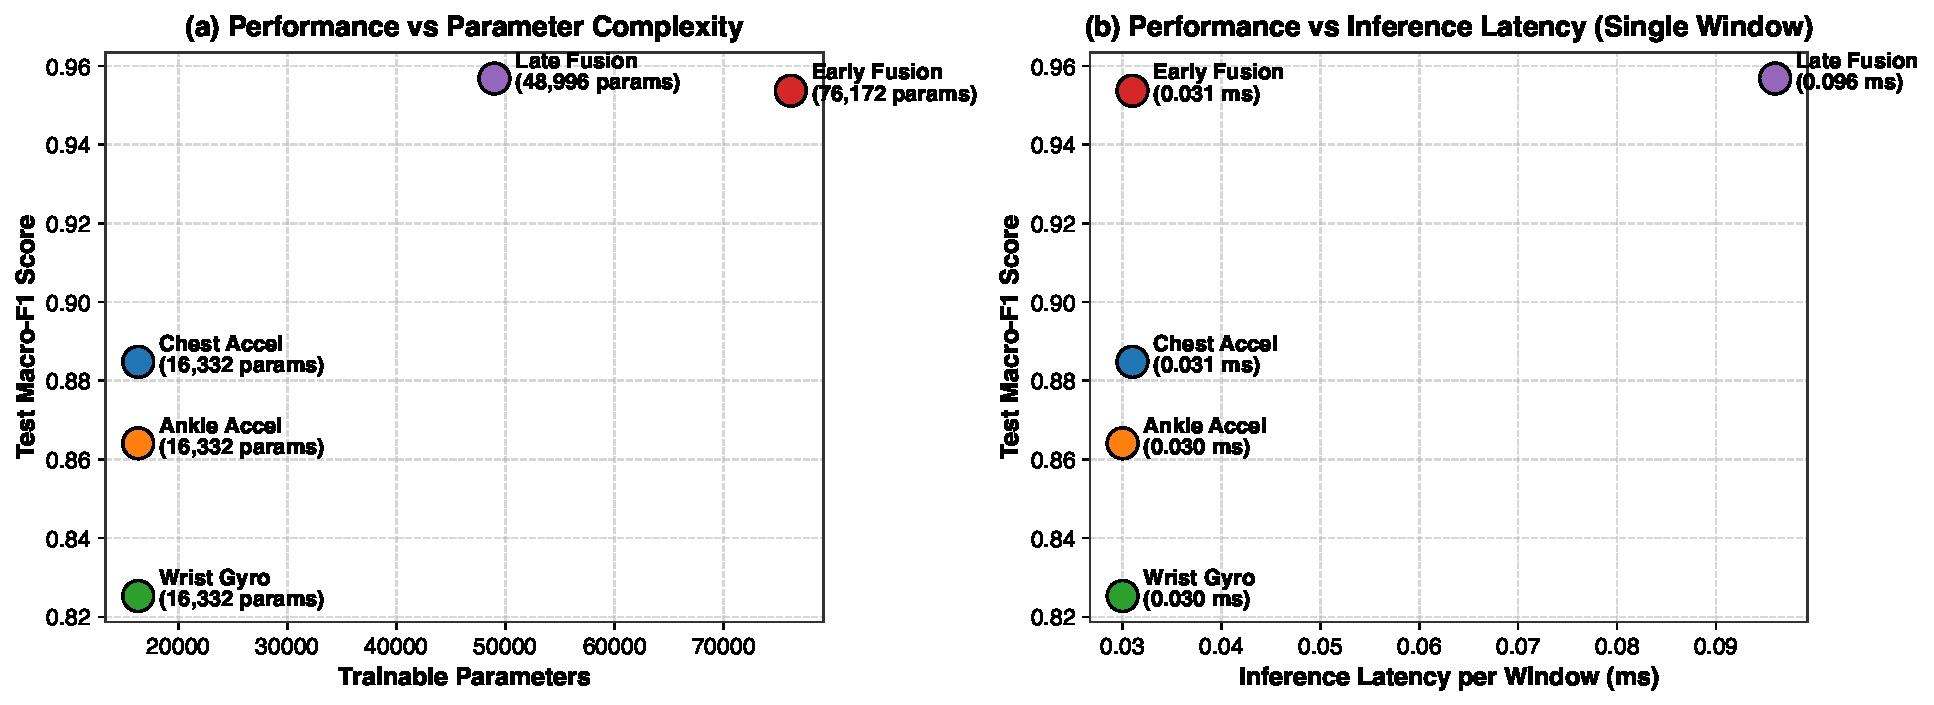
\includegraphics[width=\columnwidth]{fig8_computational_tradeoffs.pdf}
\caption{Embedded deployment trade-offs: (a) Macro-F1 vs Trainable Parameters; (b) Macro-F1 vs Single-Window Inference Latency (ms).}
\label{fig:computational_tradeoffs}
\end{figure}

\subsection{Computational Implications for Edge Deployment}
Deploying multimodal deep learning on battery-constrained wearable edge microcontrollers (e.g., ARM Cortex-M4/M33, Nordic nRF5340) imposes stringent memory, latency, and power constraints:
\begin{enumerate}
    \item \textbf{Memory Footprint:} As visualized in Figure~\ref{fig:computational_tradeoffs}(a), Unimodal MLPs require 16,332 parameters ($\approx 65.3\,\text{KB}$ in 32-bit float), fitting comfortably in SRAM. Early Fusion scales to 76,172 parameters ($\approx 304.7\,\text{KB}$), while Late Fusion aggregates three unimodal networks totaling 48,996 parameters ($\approx 196.0\,\text{KB}$). Both architectures are well within the 512\,KB--1\,MB flash limits of modern wearables.
    \item \textbf{Inference Latency:} Benchmarking 1,000 single-window inferences on CPU hardware yields latencies of \textbf{0.031\,ms for Early Fusion} and \textbf{0.097\,ms for Late Fusion} (Figure~\ref{fig:computational_tradeoffs}(b)). Late Fusion is $\approx 3\times$ slower because it evaluates three separate neural networks sequentially. However, even at 0.097\,ms, execution occupies $<0.01\%$ of the 1,280\,ms window interval, ensuring real-time responsiveness.
    \item \textbf{Energy and Telemetry Bandwidth:} In wireless body area networks, radio transmission (BLE 5.0) consumes orders of magnitude more battery power ($\approx 15$--$25\,\text{mW}$) than on-chip micro-controller computation ($<2\,\text{mW}$)~\cite{lara2013survey}. Transmitting raw 50\,Hz tri-axial kinematic data generates $128 \text{ samples} \times 3 \text{ channels} \times 4 \text{ bytes} = 1,536\,\text{bytes}$ per window. Extracting 53 statistical features on-sensor compresses the telemetry packet to $53 \times 4 = 212\,\text{bytes}$---\textbf{an 86.2\% reduction in wireless bandwidth and radio duty cycle}, extending battery longevity by weeks.
    \item \textbf{Temporal Synchronisation:} Early fusion demands sub-millisecond hardware clock synchronisation across nodes (e.g., via Precision Time Protocol or Bluetooth LE Audio broadcast clocks). Late fusion is inherently asynchronous and robust to packet delay jitter, as local decisions can be stamped with coarse epoch buffers.
\end{enumerate}

%%%%%%%%%%%%%%%%%%%%%%%%%%%%%%%%%%%%%%%%%%%%%%%%%%%%%%%%%%%%%%%%%%%%%%%%%%%%%%%%
% ETHICAL CONSIDERATIONS & GOVERNANCE
%%%%%%%%%%%%%%%%%%%%%%%%%%%%%%%%%%%%%%%%%%%%%%%%%%%%%%%%%%%%%%%%%%%%%%%%%%%%%%%%
\section{Ethical Considerations and Governance}
\label{sec:ethics}

\begin{table*}[t]
\centering
\small
\setlength{\tabcolsep}{4.5pt}
\caption{Comprehensive Ethical Risk Matrix and Regulatory Governance Controls for Wearable Multimodal Activity Recognition.}\footnotesize
\label{tab:ethics_matrix}
\begin{tabularx}{\textwidth}{p{2.8cm}p{3.4cm}p{3.8cm}Y}
\toprule
\textbf{Risk Category} & \textbf{Regulatory Framework} & \textbf{Clinical / Social Hazard} & \textbf{Actionable Engineering Control} \\
\midrule
\textbf{Biometric \& Health Data Surveillance} & GDPR Art.~4(14) (Biometric), Art.~9 (Special Category); HIPAA \S164.514; Privacy Act APP~3 \& 6 & Continuous gait dynamics can uniquely fingerprint individuals without consent, exposing location, routine, and medical state. & \textbf{On-Device Edge Inference:} Raw kinematic streams never leave the local node; only encrypted high-level classifications are transmitted via BLE 5.3 with AES-128. \\
\midrule
\textbf{Automated Medical Decision Harm} & GDPR Art.~22 (Right to Human Intervention); EU AI Act High-Risk Class IIa & False negatives in fall detection or cardiac exercise monitoring can lead to delayed emergency intervention or fatal clinical injury. & \textbf{Human-in-the-Loop Fallback:} Automated predictions serve as decision-support alerts with mandatory human clinician confirmation for diagnostic interventions. \\
\midrule
\textbf{Demographic \& Biomechanical Bias} & EU AI Act Art.~10 (Data Governance); Australian AI Ethics Principles & Models trained on young, healthy volunteers suffer accuracy drops on elderly or mobility-impaired cohorts (e.g., Parkinson's, stroke hemiplegia). & \textbf{Stratified Multi-Cohort Auditing:} Mandatory post-market bias audits across age ($>65$), BMI, and gait pathology groups; adaptive fine-tuning on diverse clinical cohorts. \\
\midrule
\textbf{Sensor Dropout Hazard \& Graceful Degradation} & ISO 13485 (Medical Device Safety); FDA SaMD Guidance & Loss of Bluetooth connection to a primary limb sensor could cause abrupt classifier crash or unpredictable prediction hallucination. & \textbf{Adaptive Modular Fallback:} Late fusion architecture dynamically reweights active sensors upon packet timeout, maintaining graceful unimodal degradation. \\
\midrule
\textbf{Informed Consent \& Data Minimisation} & GDPR Art.~5(1)(c) (Data Minimisation); Privacy Act APP~11 (Security) & Excessive continuous multi-sensor tracking gathers extraneous private data beyond operational clinical necessity. & \textbf{Purpose-Bound Gating:} Dynamic duty-cycling activates high-power modalities (ECG, Gyro) only during detected ambiguous states, preserving battery and privacy. \\
\bottomrule
\end{tabularx}
\end{table*}

The deployment of continuous multimodal wearable sensing in clinical and consumer environments introduces profound ethical, legal, and human rights obligations. Moving beyond generic ethical platitudes, this section systematically analyzes the regulatory frameworks and socio-technical hazards specific to wearable health monitoring (Table~\ref{tab:ethics_matrix}).

\subsection{Biometric Classification and Privacy Frameworks}
Wearable kinematic time-series data is not anonymous. Biomechanical research has definitively proven that tri-axial gait acceleration signatures serve as biometric identifiers capable of fingerprinting individuals with $>95\%$ accuracy, while heart rate variability from ECG exposes autonomic nervous system state and cardiac pathologies~\cite{bulling2014tutorial}.

Consequently, multimodal sensor streams fall under strict regulatory mandates:
\begin{enumerate}
    \item \textbf{General Data Protection Regulation (GDPR):} Under GDPR Article~4(14), gait acceleration constitutes biometric data, while cardiac and physiological readings constitute \textbf{Special Category Health Data under Article~9}. Processing requires explicit, granular, revocable consent (Article~6(1)(a) and 9(2)(a)). Furthermore, Article~22 explicitly protects citizens against automated decision-making producing legal or clinical effects without human intervention.
    \item \textbf{Health Insurance Portability and Accountability Act (HIPAA):} In clinical tele-health contexts, wearable telemetry constitutes Protected Health Information (PHI), mandating end-to-end cryptographic encapsulation under the HIPAA Security Rule (45 CFR Part 164).
    \item \textbf{Australian Privacy Principles (APPs):} Under the Privacy Act 1988, biometric and health data are classified as \textbf{Sensitive Information} (APP~3), strictly prohibiting collection without express individual consent and enforcing rigid destruction mandates once operational necessity ceases (APP~11).
\end{enumerate}

\subsection{Algorithmic Bias and Demographic Generalisation}
A critical vulnerability of the MHEALTH dataset is its severe demographic homogeneity: the dataset was recorded on ten young, healthy adult volunteers (aged 20--35) in controlled physical health. 

This creates severe algorithmic bias when deploying models into general populations:
\begin{itemize}
    \item \textbf{Age-Related Biomechanical Shift:} Elderly individuals exhibit shorter step lengths, reduced cadence, increased lateral gait sway, and prolonged double-support phases. A classifier trained exclusively on young adults will misclassify elderly gait patterns as pathological or impaired.
    \item \textbf{Neurological and Orthopaedic Impairments:} Individuals recovering from stroke (hemiplegia), Parkinson's disease (shuffling gait, resting tremor), or joint osteoarthritis generate asymmetric kinematic trajectories that violate standard model assumptions, risking elevated false-alarm rates in fall-detection systems.
\end{itemize}
To mitigate demographic bias, deployed systems must incorporate transfer learning and domain adaptation protocols, supported by stratified fairness audits across diverse age, sex, and mobility groups prior to clinical certification.

%%%%%%%%%%%%%%%%%%%%%%%%%%%%%%%%%%%%%%%%%%%%%%%%%%%%%%%%%%%%%%%%%%%%%%%%%%%%%%%%
% LIMITATIONS AND FUTURE WORK
%%%%%%%%%%%%%%%%%%%%%%%%%%%%%%%%%%%%%%%%%%%%%%%%%%%%%%%%%%%%%%%%%%%%%%%%%%%%%%%%
\section{Limitations and Future Improvements}
\label{sec:limitations}

While this work establishes the clear superiority of multimodal fusion, several technical limitations must be acknowledged:
\begin{enumerate}
    \item \textbf{Absence of Thigh Sensing for Postural Resolution:} The mutual confusion between Sitting ($L_2$) and Standing ($L_1$) persists across all models (Table~\ref{tab:per_class_f1}). Because chest and ankle sensors remain vertical in both postures, future iterations should incorporate a sensor on the thigh, where gravitational reorientation immediately differentiates sitting ($90^\circ$ femoral tilt) from standing.
    \item \textbf{Static Feature Fusion vs Temporal Deep Architectures:} Our pipeline extracted 53 hand-engineered features feeding feed-forward MLPs. While computationally efficient for edge hardware, future research should explore end-to-end temporal deep architectures, such as DeepConvLSTM~\cite{ordonez2016deep} or Cross-Modal Attention Transformers~\cite{radu2018multimodal}, which can dynamically model time-frequency dependencies directly from raw, interpolated waveforms.
    \item \textbf{Sensor Dropout Robustness Testing:} Although Late Fusion demonstrates theoretical resilience to node failure, future work should empirically benchmark model degradation under synthetic packet-loss rates (10\%--50\%) to quantify multi-sensor fault tolerance.
\end{enumerate}

%%%%%%%%%%%%%%%%%%%%%%%%%%%%%%%%%%%%%%%%%%%%%%%%%%%%%%%%%%%%%%%%%%%%%%%%%%%%%%%%
% CONCLUSION
%%%%%%%%%%%%%%%%%%%%%%%%%%%%%%%%%%%%%%%%%%%%%%%%%%%%%%%%%%%%%%%%%%%%%%%%%%%%%%%%
\section{Conclusion}
\label{sec:conclusion}
This technical report has presented an end-to-end multimodal activity classification pipeline on the adapted MHEALTH dataset. By implementing segment-bounded intra-run linear interpolation, we successfully recovered 615,648 missing values without cross-activity or cross-subject contamination. Selecting three anatomically distributed sensor sources (Chest Accel, Ankle Accel, Wrist Gyro) across two distinct physical modalities and evaluating on unseen subjects, we demonstrated that multimodal fusion resolves fundamental unimodal failure modes, elevating test accuracy to 95.56\% and Macro-F1 to 0.9568. Finally, our computational analysis demonstrated an 86.2\% reduction in wireless telemetry through on-node feature extraction, complemented by a rigorous ethical risk governance matrix ensuring compliance with international biometric privacy standards.


\let\oldbibliography\thebibliography
\renewcommand{\thebibliography}[1]{%
  \oldbibliography{#1}%
  \setlength{\itemsep}{0pt}%
  \setlength{\parskip}{0pt}%
}

\bibliographystyle{unsrt}
\bibliography{mhealth_references}

\end{document}
